% =====================================================================
%  c08 —— PDF p.64–69（原书 p.58–63）
%  §3.4 M̄_{g,n} 的相交理论
% =====================================================================

% ===== 原书 p.58 =====
% （本页开头一句「称 ω 为 BU(1)^{comb} 的万有基本形式，u_1 为……万有基本类。」
%   已由 c07 译完，本块自此段起译。）
现在，对$i=1,\dots,n$，设
\[
\partial_i:\Mbar^{comb}_{g,n}\longrightarrow BU(1)^{comb}
\]
为把各边界的带编号图与之对应的映射。此时$\partial_i$诱导出上同调之间的映射
\[
\partial_i^*:H^*_{DR}(BU(1)^{comb})\longrightarrow H^*_{DR}(\Mbar^{comb}_{g,n}),
\]
并把$u_1$在$\partial_i^*$下的像记作$c_i$（$i=1,\dots,n$）。又由 de Rham 定理，把与$u_i$对应的$H^i(\MbarGN)$的元素记作$c_{i,sing}$。

\transnote{原文此句写「与$u_i$对应的$H^i(\MbarGN)$的元素」，但前文只定义了$u_1$（即$H^2_{DR}(BU(1)^{comb})$的元素），$H$的次数也应为$2$；此处照原文译出。}

\subsection{$\MbarGN$的相交理论}

由 Deligne–Mumford 的可表示性，$\MbarGN$在代数意义下具有平展且可表示的覆盖$X_0$。把其伴随解析空间记作$X_0^{an}$。现在，对于$x=(C,p_1,\dots,p_n,r_1,\dots,r_n)\in X_0^{an}\times\R_+^n$，考虑$C_v$（$v\in V_{nc}$）上具有闭轨道且满足下述条件的二次微分$\omega$：
\begin{enumerate}[label=(\arabic*)]
\item 若$p_i\in C_v$，则关于由$\omega_v$确定的度量，$p_i$周围的闭轨道的长度为$r_i$。
\item 特征环域仅为$p_i$周围的小闭曲线。
\item 对属于$C_v$的$C$的奇点，$\omega_v$具有至多$1$阶极点。
\end{enumerate}
由此得到的带度量的稳定带状图记作$(\Gamma_x,G_x(v))$。此时，设$X_0^{an}\times\R_+^n$有足够细的覆盖$X_0^{an}\times\R_+^n=\cup U_k$，且满足下述条件。在各$U_k$上，$\{G_x(v)\}_v$的第$i$个边界上定有连续的标架。不过这里所说的连续标架，也允许退化的情形。

% ===== 原书 p.59 =====
即，也允许下面那样的标架。

\begin{center}
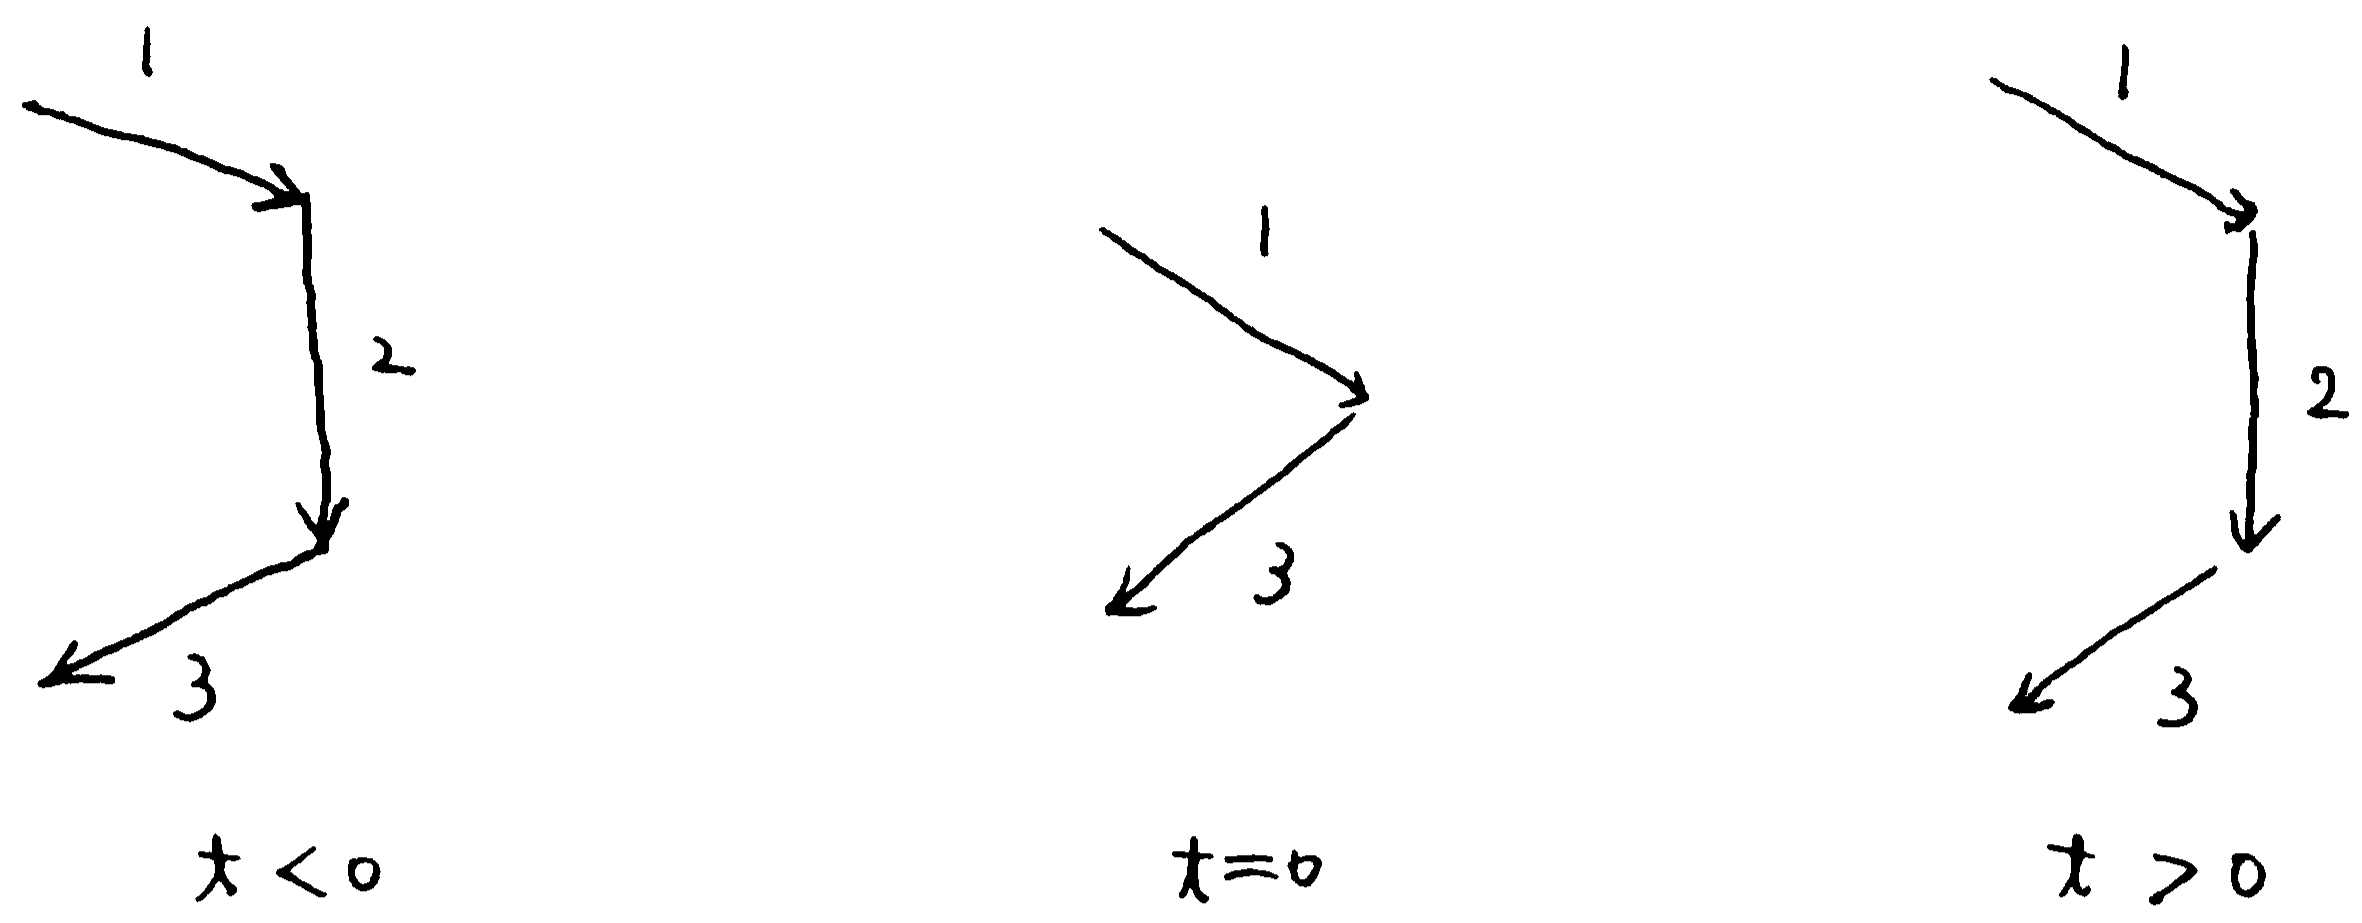
\includegraphics[width=0.62\linewidth]{fig_p65_a.png}
\end{center}

对各个$U_i$固定一个边界的标架，由此定义连续映射
\[
\coprod U_i\longrightarrow(\Mbar^{comb}_{g,n})_0.
\]
重新置$Y_0=\coprod U_i$，并置$Y_1=Y_0\times_{(\MbarGN\times\R_+^n)^{an}}Y_0$，则$Y_1$到$(\Mbar^{comb}_{g,n})_1$自然诱导出连续映射，故作为余等化子的映射
\[
f:\Mbar^{an}_{g,n}\times\R_+^n\longrightarrow\Mbar^{comb}_{g,n}
\]
被定义。由此，经由到单纯空间的诱导映射，可定义奇异同调、奇异上同调的映射
\[
\begin{aligned}
H_*(\MbarGN\times\R_+^n,\Q)&\xrightarrow{f_*}H_*(\Mbar^{comb}_{g,n},\Q),\\
H^*(\Mbar^{comb}_{g,n},\Q)&\xrightarrow{f^*}H^*(\MbarGN\times\R_+^n,\Q).
\end{aligned}
\]
在 de Rham 上同调中，类似的映射也被预期可以诱导出来，但因稍难理解，此处不作讨论。现在，把$\MbarGN$上的线丛$s_i^*(T_{\mathcal{C}/\MbarGN})$记作$\mathcal{L}_i$。这里$\mathcal{C}\to\MbarGN$为万有曲线。此时，$\mathcal{L}_i$的 Chern 类$c_1(\mathcal{L}_i)$定在$H^2(\MbarGN,\R)$中。进一步此时，

\begin{proposition}
\[
f^*(c_{i,sing})=pr_1^*\bigl(c_1(\mathcal{L}_i)\bigr).
\]
\end{proposition}

这里$\mathrm{pr}_1^*$是自然诱导映射
\[
\mathrm{pr}_1^*:H^*(\MbarGN,\R)\longrightarrow H^*(\MbarGN\times\R_+^n,\R).
\]

% ===== 原书 p.60 =====
现在固定$\mathbf{r}=(r_1,\dots,r_r)\in\R_+^n$，考虑包含映射
\[
i_{\mathbf{r}}:\MbarGN\hookrightarrow\MbarGN\times\R_+^n;\quad x\mapsto(x,\mathbf{r}).
\]
则$\mathrm{pr}_1\circ i_{\mathbf{r}}=\id$。因$\dim\MbarGN=6g-6+2n$，故当$d_1+\cdots+d_n=3g-3+n$时，有$c_1(\mathcal{L}_1)^{d_1}\wedge\cdots\wedge c_1(\mathcal{L}_n)^{d_n}\in H^{6g-6+2n}(\MbarGN,\Q)$，从而
\[
\tr_{\MbarGN}\bigl(c_1(\mathcal{L}_1)^{d_1}\wedge\cdots\wedge c_1(\mathcal{L}_n)^{d_n}\bigr)\in\Q .
\]

\transnote{原文此处写$\mathbf{r}=(r_1,\dots,r_r)\in\R_+^n$，最后一个下标与前面的$r_1$不一致，疑应为$r_n$；此处照原文译出。}

迹映射$H^{6g-6+2n}(\MbarGN,\Q)\to\Q$与$H_{6g-6+2n}(\MbarGN,\Q)\ni[\MbarGN]$的自然配对一致，故
\[
\begin{aligned}
&\tr_{\MbarGN}\bigl(c_1(\mathcal{L}_1)^{d_1}\wedge\cdots\wedge c_1(\mathcal{L}_n)^{d_n}\bigr)\\
&\quad=\bigl([\MbarGN],c_1(\mathcal{L}_1)^{d_1}\wedge\cdots\wedge c_1(\mathcal{L}_n)^{d_n}\bigr)\\
&\quad=\bigl([\MbarGN],i_{\mathbf{r}}^*pr_1^*\bigl(c_1(\mathcal{L}_1)^{d_1}\wedge\cdots\wedge c_1(\mathcal{L}_n)^{d_n}\bigr)\bigr)\\
&\quad=\bigl(i_{\mathbf{r},*}[\MbarGN],(pr_1^*c_1(\mathcal{L}_1))^{d_1}\wedge\cdots\wedge(pr_1^*c_1(\mathcal{L}_n))^{d_n}\bigr)\\
&\quad=\bigl(i_{\mathbf{r}*}[\MbarGN],(f^*c_1)^{d_1}\wedge\cdots\wedge(f^*c_n)^{d_n}\bigr)\\
&\quad=\bigl(f_*i_{\mathbf{r},*}[\MbarGN],c_1^{d_1}\wedge\cdots\wedge c_n^{d_n}\bigr)
\end{aligned}
\]
成立。现在置$f_*i_{\mathbf{r},*}[\MbarGN]=[\Mbar^{comb}_{g,n}]$，构造代表$[\Mbar^{comb}_{g,n}]$的闭链$\Mbar^{comb}_{g,n}$。若能办到，则由$\Mbar^{comb}_{g,n}$处的 de Rham 定理，
\[
\bigl(f_*i_{\mathbf{r},*}[\MbarGN],c_1^{d_1}\wedge\cdots\wedge c_n^{d_n}\bigr)
=\int_{\Mbar^{comb}_{g,n}}c_1^{d_1}\wedge\cdots\wedge c_n^{d_n}
\]
成立。现在，设$TG_{g,n}$为亏格$g$、边界个数为$n$的三价带状图（但边界已编号）的集合。对$TG_{g,n}$的每个元素$G$，各边界上的标架各取一个，以下固定此标架。对$G$，令$\Delta_{G,\mathbf{r}}$为使$G$的度量中$p_i$处的边界长度为$r_i$的度量的全体。利用$G$为三价这一点，其边数为$6g-6+3n$。故$\Delta_{G,\mathbf{r}}$是$\R_+^{6g-6+3n}$内的$(6g-6+2n)$维多面体。对此，亏格$g$的

% ===== 原书 p.61 =====
$n$点 Riemann 面的族$C_{G,\mathbf{r}}$在$\Delta_{G,\mathbf{r}}$上构成，由此定出$\Delta_{G,\mathbf{r}}$到$\MbarGN$的映射。现在，设$U\to T$为$Aut(G)$-主丛，且给定等变映射$U\to\Delta_{G,\mathbf{r}}$，则把$\Delta_{G,\mathbf{r}}$上的 Riemann 面的族$C_{G,\mathbf{r}}$拉回到$U$上，其上便诱导出$G$的作用。由于此作用自由，可得$T$上的 Riemann 面的族。即，
\[
\bigl[\Delta_{G,\mathbf{r}}/Aut(G)\bigr]\longrightarrow\MbarGN
\]
的映射被定义。且此映射成为单射。由此可知，$\sum_{G\in TG_{g,n}}\frac{1}{Aut(G)}\Delta_{g,n}$是$[\MbarGN]\in H_{6g-6+2n}(\MbarGN)$的代表。又可知，它自然给出$\Mbar^{comb}_{g,n}$的$(6g-6+2n)$维闭链。把它置作$\Mbar^{comb}_{g,n,\mathbf{r}}$，则由$i_{\mathbf{r}}$的定义得$f_*i_{\mathbf{r},*}[\MbarGN]=[\Mbar^{comb}_{g,n,\mathbf{r}}]$。

(1)
\[
\Mbar^{comb}_{g,n,\mathbf{r}}=\sum_{G\in TG_{g,n}}\frac{1}{Aut(G)}\Delta_{G,\mathbf{r}}
\]

把(1)、(2)合起来，得到下面的定理。

\transnote{原文此处引用 (2)，但本页及前页只给 (1) 编了号，上一页中迹与相交数相等的等式链并未编号；此处照原文译出。}

\begin{theorem}
\[
\langle\tau_{d_1},\dots,\tau_{d_n}\rangle
=\sum_{G\in TG_{g,n}}\frac{1}{Aut(G)}\int_{\Delta_{G,\mathbf{r}}}c_1^{d_1}\wedge\cdots\wedge c_n^{d_n}
\]
\end{theorem}

这里
\[
c_i=\sum_{1\le j\le k\le N_i-1}d\Bigl(\frac{l_k}{r_i}\Bigr)\wedge d\Bigl(\frac{l_j}{r_i}\Bigr),
\]
$N_i$为边界$\partial_i$的个数，$l_1,\dots,l_{N_i}$为按$G$的标架的顺序排列的、出现在$\partial_i$中的边的长度。

由此，相交数完全用组合的数表出。此处，在开始计算右端之前，先对$\mathbf{r}$作 Radon 变换。设$f(\mathbf{r})=f(r_1,\dots,r_n)$为$\R_+^n$上可积的函数。由上述定理 3.5 与 Fubini 定理，
\[
\begin{aligned}
&\Bigl(\int_{\R_+^n}f(\mathbf{r})dr_1\wedge\cdots\wedge dr_n\Bigr)
\langle\tau_{d_1},\dots,\tau_{d_n}\rangle\\
&\quad=\sum_{G\in TG_{g,n}}\frac{1}{Aut(G)}
\int_{\Delta_G}f(\mathbf{r})c_1^{d_1}\wedge\cdots\wedge c_n^{d_n}\wedge dr_1\wedge\cdots\wedge dr_n
\end{aligned}
\]

% ===== 原书 p.62 =====
成立。这里$\Delta_G$为$G$的全部度量的全体，经$G$的边界的标架与$\R_+^{6g-6+2n}$等同。现在，取$\lambda_1,\dots,\lambda_n\in\R$，对
\[
f(\mathbf{r})=\prod_i\frac{1}{d_i!}\exp(-\lambda_1r_1-\cdots-\lambda_nr_n)r_1^{2d_1}\cdots r_n^{2d_n}
\]
应用上式，再对满足$d_1+\cdots+d_n=3g-3+n$、$d_1\ge0,\dots,d_n\ge0$的$d_1,\dots,d_n$求和，便得下述等式。

\begin{proposition}
\[
\begin{aligned}
&\sum_{d_1+\cdots+d_n=3g-3+n}\prod_i\frac{1}{d_i!}\langle\tau_{d_1},\dots,\tau_{d_n}\rangle\\
&\qquad\times\int\exp(-\lambda_1r_1-\cdots-\lambda_nr_n)r_1^{2d_1}\cdots r_n^{2d_n}dr_1\wedge\cdots\wedge dr_n\\
&=\sum_{G\in TG_{g,n}}\frac{1}{d!Aut(G)}\int_{\Delta_G}\exp(-\lambda_1r_1-\cdots-\lambda_nr_n)\\
&\qquad\times(r_1^2c_1+\cdots+r_n^2c_n)^d dr_1\wedge\cdots\wedge dr_n
\end{aligned}
\]
\end{proposition}

其次，把两边看作关于$\lambda_1,\dots,\lambda_n$的函数等式。先看左边，利用等式
\[
\int_0^\infty\exp(-\lambda r)r^{2d}dr=\frac{(2d)!}{\lambda^{2d+1}}
\]
可得
\[
\sum_{d_1+\cdots+d_n=3g-3+n}\langle\tau_{d_1},\dots,\tau_{d_n}\rangle
\prod_{i=1}^n\frac{(2d_i-1)!!}{\lambda_i^{2d_i+1}}.
\]
计算右边需要下面的引理。

\begin{lemma}[Kontsevich {[K]}，定理 C.1]
置$\Omega=\sum_{i=1}^nr_i^2c_i$，则
\[
\frac{\Omega^d}{d!}dr_1\wedge\cdots\wedge dr_n=2^{5g-5+2n}\prod_{e\in G^{(1)}}dl_e
\]
成立。这里$G^{(1)}$为$G$的边的集合。
\end{lemma}

证明从略。利用上述引理 3.7，命题 3.6 的右端可表为
\[
\begin{aligned}
&\sum_{G\in TG_{g,n}}\frac{2^{5g-5+2n}}{Aut(G)}
\int_{\Delta_G}\exp(-\lambda_1r_1-\cdots-\lambda_nr_n)\prod_{e\in G^{(1)}}dl_e\\
&=\sum_{G\in TG_{g,n}}\frac{2^{-4g+4-2n}}{Aut(G)}\prod_{e\in G^{(1)}}\frac{2}{\tilde\lambda(e)}.
\end{aligned}
\]
这里，当$e\in G^{(1)}$为边界$\partial_i$与$\partial_j$的一部分时，定义$\tilde\lambda(e)=\lambda_i+\lambda_j$。把以上全部综合，便得下面的定理。

% ===== 原书 p.63 =====
\begin{theorem}[Main identity]
\[
\sum_{d_1+\cdots+d_n=3g-3+n}\langle\tau_{d_1},\dots,\tau_{d_n}\rangle
\prod_{i=1}^n\frac{(2d_i-1)!!}{\lambda_i^{2d_i+1}}
=\sum_{G\in TG_{g,n}}\frac{2^{-4g+4-2n}}{Aut(G)}\prod_{e\in G^{(1)}}\frac{2}{\tilde\lambda(e)}
\]
\end{theorem}
